% ============================================================
%  THGNN Presentation — Financial Time Series Forecasting
%  Beamer / metropolis theme
%
%  Diagram workflow
%  ----------------
%  Five architecture diagrams live in diagrams/*.drawio.
%  Edit them in draw.io, export each as PDF (File → Export as → PDF,
%  tick "Fit page") and place next to the .drawio files in
%  presentation/diagrams/.  The \drawioimg guards pick them up
%  automatically; until then a placeholder box is shown.
% ============================================================
\documentclass[aspectratio=169, 10pt]{beamer}

% ---- Theme --------------------------------------------------
\usetheme{metropolis}
\usepackage{appendixnumberbeamer}

% ---- Packages -----------------------------------------------
\usepackage{booktabs}
\usepackage{amsmath, amssymb}
\usepackage{mathtools}
\usepackage{graphicx}
\usepackage{xcolor}
\usepackage{tikz}
\usetikzlibrary{shapes.geometric, arrows.meta, positioning, fit, backgrounds, calc}
\usepackage{pgfplots}
\pgfplotsset{compat=1.18}
\usepackage{hyperref}
\usepackage{multirow}
\usepackage{array}
\usepackage{colortbl}

% ---- Colour palette (light-blue scheme) ---------------------
\definecolor{primary}{HTML}{1976D2}   % Material Blue 700 — frame titles
\definecolor{accent}{HTML}{5DADE2}    % sky blue — progress bar, links
\definecolor{positive}{HTML}{1E8449}  % green
\definecolor{negative}{HTML}{C0392B}  % red
\definecolor{neutral}{HTML}{7F8C8D}   % grey
\definecolor{highlight}{HTML}{F39C12} % amber
\definecolor{lightbg}{HTML}{E3F2FD}   % Material Blue 50 — block bodies
\definecolor{darkbg}{HTML}{1A252F}

\setbeamercolor{palette primary}{bg=primary, fg=white}
\setbeamercolor{frametitle}{bg=primary, fg=white}
\setbeamercolor{progress bar}{fg=accent}
\setbeamercolor{alerted text}{fg=highlight}
\setbeamercolor{block title}{bg=primary, fg=white}
\setbeamercolor{block body}{bg=lightbg}
\setbeamercolor{alerted text}{fg=highlight}
\setbeamercolor{block title alerted}{bg=negative, fg=white}
\setbeamercolor{block body alerted}{bg=negative!10}

% ---- Global list spacing (prevents overflow) ----------------
\setlength{\itemsep}{3pt}
\setlength{\parskip}{2pt}

% ---- Metadata -----------------------------------------------
\title{Financial Time Series Forecasting\\with Graph Neural Networks}
\subtitle{THGNN: Temporal and Heterogeneous GNN for Nifty 50 Stock Prediction}
\author{Debarshi Chakraborty}
\date{\today}
\institute{Financial Time Series Forecasting Project}

% ---- Custom commands ----------------------------------------
\newcommand{\myvec}[1]{\mathbf{#1}}
% Checkmark / cross without fontawesome
\newcommand{\cmark}{\textcolor{positive}{\textbf{\checkmark}}}
\newcommand{\xmark}{\textcolor{negative}{\textbf{\texttimes}}}

% Helper: include draw.io-exported PDF if it exists, else placeholder
\newcommand{\drawioimg}[3][width=\textwidth]{%
  \IfFileExists{diagrams/#2.pdf}{%
    \includegraphics[#1]{diagrams/#2.pdf}%
  }{%
    \begin{tikzpicture}
      \node[draw=neutral, dashed, fill=lightbg, rounded corners,
            minimum width=0.95\linewidth, minimum height=3.2cm,
            align=center, font=\small\itshape, text=neutral]
        {#3\\[4pt]\footnotesize\ttfamily
         Export diagrams/#2.drawio from draw.io as PDF};
    \end{tikzpicture}%
  }%
}

% ============================================================
\begin{document}

\maketitle

% ---- Table of Contents --------------------------------------
\begin{frame}{Outline}
  \setbeamertemplate{section in toc}[sections numbered]
  \tableofcontents[hideallsubsections]
\end{frame}

% ============================================================
\section{Motivation \& Problem Statement}
% ============================================================

\begin{frame}{The Stock Ranking Problem}
  \begin{columns}[T]
    \begin{column}{0.55\textwidth}
      \textbf{Goal:} Given $N$ stocks over $T$ days, predict their
      \emph{relative cross-sectional ranking} at $t{+}1$.

      \medskip
      \textbf{Key challenges:}
      \begin{itemize}\setlength{\itemsep}{2pt}
        \item Market is non-stationary and noisy
        \item Stocks are \alert{not independent} — sector shocks, macro events
        \item Relationships are \alert{dynamic}: correlations change over time
        \item Pure MSE does not align with portfolio objectives
      \end{itemize}

      \medskip
      \textbf{Evaluation:} Information Coefficient (IC)
      $= \text{Spearman}(\hat{r}, r)$\\
      \quad IC $>0.05$ is practically useful;\quad IC $>0.10$ is strong.
    \end{column}
    \begin{column}{0.42\textwidth}
      \begin{block}{Task Definition}
        \textbf{Input:} $\myvec{X} \in \mathbb{R}^{N \times T \times F}$\\
        \quad $N=50$ stocks (Nifty 50)\\
        \quad $T=20$ trading-day look-back\\
        \quad $F=12$ features (see Data Pipeline)
        \smallskip\\
        \textbf{Output:} $\hat{\myvec{r}} \in \mathbb{R}^{N}$\\
        \quad Predicted next-day return per stock
        \smallskip\\
        \textbf{Objective:}
        $\max\;\text{Spearman}(\hat{\myvec{r}},\, \myvec{r}_{t+1})$
      \end{block}
    \end{column}
  \end{columns}
\end{frame}

\begin{frame}{Why Graph Neural Networks?}
  \begin{center}
  \drawioimg[width=0.62\textwidth, keepaspectratio]%
    {03_stock_correlation_graph}%
    {Stock Correlation Graph}%
  \end{center}
  \vspace{-0.3cm}
  \begin{block}{}
    A graph representation allows the model to \textbf{propagate information}
    across correlated stocks — a fundamental advantage over treating each
    stock independently.
  \end{block}
\end{frame}

% ============================================================
\section{Literature Review \& Model Evolution}
% ============================================================

\begin{frame}{Evolution of Stock Prediction Architectures}
  \drawioimg[width=\textwidth, height=0.72\textheight, keepaspectratio]%
    {04_architecture_evolution}%
    {Architecture Evolution: MASTER / StockMixer → THGNN → Hypergraph}

  \smallskip
  This work implements \alert{THGNN}, the first step towards relational
  stock modelling, and analyses the path toward hypergraph architectures.
\end{frame}

\begin{frame}{MASTER \& StockMixer — Strengths and Gaps}
  \begin{columns}[T]
    \begin{column}{0.48\textwidth}
      \textbf{MASTER}
      \begin{itemize}\setlength{\itemsep}{1pt}
        \item Market-index signal gates each stock's temporal features
        \item Sophisticated temporal attention for intra-stock dynamics
        \item[\xmark] \textcolor{negative}{Static or no inter-stock graph}
        \item[\xmark] \textcolor{negative}{Homogeneous relationship treatment}
      \end{itemize}
      \smallskip
      \textbf{StockMixer}
      \begin{itemize}\setlength{\itemsep}{1pt}
        \item Patch-based temporal encoding captures multi-scale trends
        \item Indicator mixing across feature channels
        \item[\xmark] \textcolor{negative}{Stocks remain independent}
        \item[\xmark] \textcolor{negative}{No relational information flow}
      \end{itemize}
    \end{column}
    \begin{column}{0.48\textwidth}
      \begin{alertblock}{Core Gap Addressed by THGNN}
        Both models process each stock's signals \emph{in isolation}.
        Real markets exhibit strong cross-stock dependencies that cannot
        be captured without explicit graph structure.
      \end{alertblock}
      \smallskip
      \textbf{THGNN's answers:}
      \begin{enumerate}\setlength{\itemsep}{2pt}
        \item Day-specific correlation graph (dynamic, not static)
        \item Separate \textcolor{positive}{positive} and
              \textcolor{negative}{negative} GAT heads (heterogeneous)
        \item Semantic attention: self vs.\ positive vs.\ negative neighbours
      \end{enumerate}
    \end{column}
  \end{columns}
\end{frame}

\begin{frame}{Beyond THGNN — The Hypergraph Frontier}
  \begin{columns}[T]
    \begin{column}{0.50\textwidth}
      \textbf{Standard GNN limitation (THGNN):}
      \begin{itemize}\setlength{\itemsep}{2pt}
        \item Edges are \emph{pairwise} only: $e = (u, v)$
        \item Cannot represent group shocks natively\\
              (e.g.\ an entire sector reacting to one event)
        \item Decomposing groups into pairs loses higher-order signal
      \end{itemize}
      \smallskip
      \textbf{Hypergraph solution:}
      \begin{itemize}\setlength{\itemsep}{2pt}
        \item \textbf{Hyperedge} $e \subseteq V$: any subset of stocks
        \item \textbf{MaGNet}: probabilistic hyperedges with soft membership
        \item \textbf{STHAN-SR}: reformulates as \emph{learning-to-rank}
              for direct profit optimisation
      \end{itemize}
    \end{column}
    \begin{column}{0.46\textwidth}
      \drawioimg[width=\textwidth, keepaspectratio]%
        {05_standard_vs_hypergraph}%
        {Standard Graph vs Hypergraph}
    \end{column}
  \end{columns}
\end{frame}

% ============================================================
\section{THGNN Architecture}
% ============================================================

\begin{frame}{THGNN — End-to-End Architecture Overview}
  \drawioimg[width=\textwidth, height=0.65\textheight, keepaspectratio]%
    {01_thgnn_pipeline}%
    {THGNN End-to-End Pipeline}

  \vspace{0.1cm}
  \begin{columns}[T]
    \begin{column}{0.50\textwidth}
      \small Each forward pass processes \textbf{one trading day} as a graph
      of 50 stock nodes.
    \end{column}
    \begin{column}{0.46\textwidth}
      \small Output: scalar \emph{predicted return} per stock for ranking.
    \end{column}
  \end{columns}
\end{frame}

% ---- Changes vs original paper ------------------------------
\begin{frame}[shrink=5]{Key Modifications from the Original THGNN Paper}
  \begin{columns}[T]
    \begin{column}{0.40\textwidth}
      \textbf{Kept from paper:}
      \begin{itemize}\setlength{\itemsep}{3pt}
        \item[\cmark] GRU temporal encoder
        \item[\cmark] Positive + Negative hetero-GAT heads
        \item[\cmark] 3-way semantic attention\\
              {\small(self / pos-neighbours / neg-neighbours)}
        \item[\cmark] Dynamic daily graph from\\
              rolling Pearson correlation
      \end{itemize}
    \end{column}
    \begin{column}{0.57\textwidth}
      \textbf{Changed or added in this work:}
      \smallskip\\
      {\small
      \renewcommand{\arraystretch}{1.2}
      \begin{tabular}{@{}ll@{}}
        \toprule
        \textbf{What} & \textbf{Why} \\
        \midrule
        LayerNorm + CS demean & remove volume dominance \& beta\\
        MLP projections after GAT & homogenise dims, non-linearity\\
        Residual skip in GAT heads & stabilise gradients\\
        \textbf{PairNorm PN-SI} & \textbf{prevent over-smoothing}\\
        \midrule
        \textbf{MSE + soft IC + dispersion} & \textbf{align loss with IC}\\
        IC warmup (0\,$\to$\,0.35, 10 ep.) & stable early training\\
        Temp.\ anneal ($\tau$: 0.19\,$\to$\,0.02) & smooth\,$\to$\,sharp ranks\\
        \midrule
        Single-horizon $t{+}1$ only & $\text{corr}(r_{t+1},r_{t+3})\approx{-}0.24$\\
        Nifty 50, $F=12$ features & Indian market + technicals\\
        \bottomrule
      \end{tabular}}
    \end{column}
  \end{columns}
  \vspace{0.15cm}
  {\footnotesize See \texttt{presentation/ARCHITECTURE\_CHANGES.md} for full technical details.}
\end{frame}
% -------------------------------------------------------------

\begin{frame}{Stage 1 \& 2 — Normalisation and Temporal Encoding}
  \begin{columns}[T]
    \begin{column}{0.48\textwidth}
      \textbf{Input Normalisation}

      \begin{block}{LayerNorm per timestep}
        \vspace{-0.4em}
        \[ \tilde{x}_{i,t} = \text{LayerNorm}_F(x_{i,t}) \]
        \vspace{-0.6em}
      \end{block}
      Prevents turnover/volume from dominating GRU gates.

      \smallskip
      \textbf{Cross-sectional demeaning}
      \textcolor{negative}{\footnotesize(added vs.\ paper)}:
      \[
        x_{i,t} \leftarrow x_{i,t} - \tfrac{1}{N}\textstyle\sum_{j=1}^N x_{j,t}
      \]
      Removes market-wide beta so the GRU focuses on stock-specific alpha.
    \end{column}
    \begin{column}{0.48\textwidth}
      \textbf{GRU Temporal Encoder}

      \begin{block}{Configuration}
        \vspace{-0.4em}
        \begin{align*}
          &\text{input\_size}=12,\quad\text{hidden}=128\\[-2pt]
          &\text{num\_layers}=1,\quad\text{dropout}=0.3
        \end{align*}
        \vspace{-0.6em}
      \end{block}

      Each stock's 20-day sequence encoded independently:
      \[
        \myvec{h}_{i,T} = \text{GRU}(\myvec{x}_{i,1:T}) \;\in\; \mathbb{R}^{128}
      \]
      Only the final hidden state $\myvec{h}_T$ is kept — a fixed-size
      summary of the full temporal context.
    \end{column}
  \end{columns}
\end{frame}

\begin{frame}[shrink=8]{Stage 3 — Heterogeneous Graph Attention (GAT)}
  \textbf{Two separate GAT heads, same node embeddings, different adjacency:}

  \vspace{0.15cm}
  \begin{center}
  \renewcommand{\arraystretch}{1.3}
  \begin{tabular}{lll}
    \toprule
    \textbf{Head} & \textbf{Adjacency mask} & \textbf{Semantics} \\
    \midrule
    \texttt{pos\_gat} & $A^+_{ij} = \mathbf{1}[\rho_{ij} > \theta]$
                      & \textcolor{positive}{Stocks moving together} \\
    \texttt{neg\_gat} & $A^-_{ij} = \mathbf{1}[\rho_{ij} < -\theta]$
                      & \textcolor{negative}{Stocks moving inversely} \\
    \bottomrule
  \end{tabular}
  \end{center}

  \vspace{0.1cm}
  \textbf{Per-head attention (additive, masked softmax):}
  \begin{align*}
    s_k &= \myvec{W}_k\,\myvec{h}
          \quad\text{(linear projection to head space)}\\[2pt]
    e_{ij}^k &= \text{LeakyReLU}\!\bigl(\myvec{w}_u^\top s_{k,i}
                + \myvec{w}_v^\top s_{k,j}\bigr)\\[2pt]
    \alpha_{ij}^k &= \frac{\exp(e_{ij}^k)\cdot A_{ij}}
                         {\sum_{\ell}\exp(e_{i\ell}^k)\cdot A_{i\ell}}
    \qquad
    \myvec{z}_i^k = \sum_j \alpha_{ij}^k\, s_{k,j}
  \end{align*}

  8 heads $\times$ 32 dim $=$ 256-dim output; residual skip-connection added
  \textcolor{negative}{\footnotesize(new vs.\ paper)}.
  Output is MLP-projected 256\,$\to$\,128 before semantic attention
  \textcolor{negative}{\footnotesize(new vs.\ paper)}.
\end{frame}

\begin{frame}{Stages 4 \& 5 — Semantic Attention and Prediction}
  \begin{columns}[T]
    \begin{column}{0.52\textwidth}
      \textbf{Semantic Attention (per-node)}

      Three 128-dim embeddings (after MLP projection):
      \[ \myvec{e}_\text{self},\;\myvec{e}_+,\;\myvec{e}_- \;\in\;\mathbb{R}^{128} \]
      Soft weights via 2-layer Tanh MLP:
      \[
        \beta_i^{(s)} = \operatorname{softmax}\!\bigl(
          \myvec{w}_2^\top \tanh(\myvec{W}_1\,\myvec{e}_i^{(s)})
        \bigr)_{s=1}^3
      \]
      \[
        \myvec{f}_i = \textstyle\sum_{s} \beta_i^{(s)}\,\myvec{e}_i^{(s)}
      \]
      Each stock independently weights self vs.\ positive vs.\ negative
      neighbours.
    \end{column}
    \begin{column}{0.45\textwidth}
      \textbf{PairNorm PN-SI}
      \textcolor{negative}{\footnotesize(added vs.\ paper)}

      Prevents over-smoothing after graph aggregation:
      \[
        \tilde{\myvec{f}}_i =
          \frac{\myvec{f}_i}{\|\myvec{f}_i\|}\cdot s \;-\;\bar{\myvec{f}}
      \]
      Keeps stock embeddings well-separated regardless of graph density.

      \medskip
      \textbf{Linear Predictor}
      \[
        \hat{r}_i = \myvec{W}_\text{pred}\,\tilde{\myvec{f}}_i \;\in\;\mathbb{R}
      \]
      No activation (regression). Xavier init at gain 0.02 keeps initial
      predictions in the $\pm 2\%$ daily-return range.
    \end{column}
  \end{columns}
\end{frame}

% ============================================================
\section{Data Pipeline}
% ============================================================

\begin{frame}{Three-Stage Data Pipeline}
  \drawioimg[width=\textwidth, height=0.48\textheight, keepaspectratio]%
    {02_data_pipeline}%
    {Three-Stage Data Pipeline}

  \smallskip
  \begin{columns}[T]
    \begin{column}{0.50\textwidth}
      \textbf{Features} ($F=12$, per stock, per day):\\[2pt]
      {\small
      \begin{tabular}{@{}ll@{}}
        \texttt{open, high, low, close} & \% change \\
        \texttt{to} (turnover), \texttt{vol} & \% change \\
        \texttt{mom5, mom10, mom20} & cumul.\ return \\
        \texttt{rsi14} & RSI-14 / 100 \\
        \texttt{vol20} & 20-day realised vol \\
        \texttt{cs\_rank} & cross-sect.\ pctile rank \\
      \end{tabular}}
    \end{column}
    \begin{column}{0.46\textwidth}
      \textbf{Graph sample shape:}\\[2pt]
      {\small
      \begin{tabular}{@{}ll@{}}
        features  & $(50,\;20,\;12)$ \\
        pos\_adj  & $(50,\;50)$ binary \\
        neg\_adj  & $(50,\;50)$ binary \\
        labels    & $(50,\;3)$ — horizons $t{+}1,2,3$ \\
      \end{tabular}}
    \end{column}
  \end{columns}
\end{frame}

\begin{frame}{Dynamic Graph Construction}
  \begin{columns}[T]
    \begin{column}{0.55\textwidth}
      \textbf{Correlation-based edge generation:}

      For each trading day $d$, Pearson correlation over the 20-day
      look-back window:
      \[
        \rho_{ij}^{(d)} = \operatorname{Pearson}\!\bigl(
          \text{close}_{i,\,d-20:d},\;
          \text{close}_{j,\,d-20:d}
        \bigr)
      \]

      Binary adjacency at threshold $\theta = 0.3$:
      \[
        A_{ij}^+ = \mathbf{1}[\rho_{ij} > \theta], \quad
        A_{ij}^- = \mathbf{1}[\rho_{ij} < -\theta]
      \]

      \begin{block}{Threshold choice}
        $\theta = 0.1$ $\to$ ${\approx}49\%$ edge density (too dense)\\
        $\theta = 0.3$ $\to$ ${\approx}15\%$ edge density (recommended)\\
        Sparser graph gives GAT meaningful structure.
      \end{block}
    \end{column}
    \begin{column}{0.42\textwidth}
      \textbf{Key design decisions:}
      \begin{enumerate}\setlength{\itemsep}{4pt}
        \item Graph \textbf{rebuilt every trading day} — captures
              time-varying correlations (crises, sector rotations)
        \item Separate $A^+$ and $A^-$ enable
              \textbf{heterogeneous} attention
        \item Forward label \textbf{purge gap}: last $h{-}1$ training
              samples dropped to prevent look-ahead leakage
        \item A 12th feature (\texttt{cs\_rank}) is appended in
              \texttt{generate\_data.py} — cross-sectional percentile
              rank of the close return
      \end{enumerate}
    \end{column}
  \end{columns}
\end{frame}

% ============================================================
\section{Training Methodology}
% ============================================================

\begin{frame}{Composite Loss Function}
  Standard MSE does not optimise for ranking.
  THGNN uses a \textbf{three-term composite loss}
  \textcolor{negative}{\footnotesize(entirely new vs.\ original paper)}:

  \begin{block}{Total Loss}
    \vspace{-0.3em}
    \[
      \mathcal{L} = \underbrace{w_\text{MSE}
        \cdot \frac{\text{MSE}(\hat{r}, r)}{\sigma_0^2}}_{\text{(1) Normalised MSE}}
      \;+\;\underbrace{w_\text{IC} \cdot (1 - \widehat{\text{IC}})}_{\text{(2) Ranking Loss}}
      \;+\;\underbrace{w_\text{disp} \cdot \mathcal{L}_\text{spread}}_{\text{(3) Dispersion}}
    \]
    \vspace{-0.3em}
  \end{block}

  \begin{columns}[T]
    \begin{column}{0.33\textwidth}
      \small\textbf{(1) MSE}\quad$w=1.0$\\
      $\sigma_0=0.01$ normalises raw MSE (${\sim}10^{-4}$) to O(1).
    \end{column}
    \begin{column}{0.33\textwidth}
      \small\textbf{(2) IC loss}\quad$w=0.35$\\
      Differentiable soft Spearman via pairwise sigmoids.
      Temperature anneals $0.19\!\to\!0.02$.
    \end{column}
    \begin{column}{0.33\textwidth}
      \small\textbf{(3) Dispersion}\quad$w=0.2$\\
      Prevents collapse or volatility:
      $\text{spread}=\hat{\sigma}/\sigma_r\in[0.2,\,2.0]$
    \end{column}
  \end{columns}

  \smallskip
  \textbf{IC Warmup:} weight ramps $0\!\to\!0.35$ over first 10 epochs
  so MSE stabilises before ranking pressure is applied.
\end{frame}

\begin{frame}{Soft Spearman IC — Differentiable Ranking}
  \begin{columns}[T]
    \begin{column}{0.55\textwidth}
      Standard Spearman rank correlation is \emph{non-differentiable}.

      \medskip
      \textbf{Soft-rank approximation:}
      \[
        \tilde{r}_i = \sum_{j \neq i}
          \sigma\!\!\left(\frac{\hat{r}_i - \hat{r}_j}{\tau}\right) + 1
      \]
      $\sigma$ = sigmoid, $\tau$ = temperature.

      \medskip
      \textbf{Temperature annealing:}
      \[
        \tau_e = \max(0.02,\; 0.2 \times 0.95^{\,e})
      \]
      \begin{itemize}\setlength{\itemsep}{2pt}
        \item \textbf{Early}: $\tau$ large $\Rightarrow$ smooth gradients
        \item \textbf{Late}: $\tau\!\to\!0.02$ $\Rightarrow$ near-discrete ranks
      \end{itemize}
    \end{column}
    \begin{column}{0.42\textwidth}
      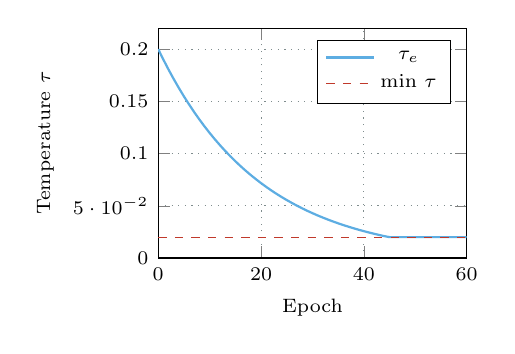
\begin{tikzpicture}
        \begin{axis}[
          width=5.5cm, height=4.5cm,
          xlabel={Epoch}, ylabel={Temperature $\tau$},
          xmin=0, xmax=60, ymin=0, ymax=0.22,
          grid=major, grid style={dotted, neutral},
          label style={font=\scriptsize},
          tick label style={font=\scriptsize},
          legend style={font=\scriptsize, at={(0.95,0.95)}, anchor=north east}
        ]
          \addplot[accent, thick, domain=0:60, samples=61]
            {max(0.02, 0.2*0.95^x)};
          \addplot[negative, dashed, domain=0:60] {0.02};
          \legend{$\tau_e$, min $\tau$}
        \end{axis}
      \end{tikzpicture}
    \end{column}
  \end{columns}
\end{frame}

\begin{frame}{Optimizer, Regularisation \& Training Protocol}
  \begin{columns}[T]
    \begin{column}{0.48\textwidth}
      \begin{center}
      \renewcommand{\arraystretch}{1.25}
      \begin{tabular}{ll}
        \toprule
        \textbf{Component} & \textbf{Setting} \\
        \midrule
        Optimizer        & AdamW \\
        Learning rate    & $10^{-4}$ \\
        Weight decay     & $10^{-3}$ \\
        Gradient clip    & $\|\nabla\|_2 \leq 1.0$ \\
        Dropout          & $0.3$ (GRU + MLPs) \\
        \midrule
        LR warmup        & 5 ep.\ ($0.1\!\times\!\to\!1\!\times$) \\
        LR schedule      & CosineAnnealingLR \\
        Early stopping   & 20 ep., val IC \\
        Max epochs       & 60 \\
        \bottomrule
      \end{tabular}
      \end{center}
    \end{column}
    \begin{column}{0.48\textwidth}
      \textbf{Data splits:}
      \begin{itemize}\setlength{\itemsep}{2pt}
        \item \textbf{Train}: 2015-01-01 – 2023-12-29 (${\sim}9$ years)
        \item \textbf{Val}:\; 2024-01-01 – 2024-12-31
        \item \textbf{Test}: 2025-01-01 – 2026-02-28
      \end{itemize}

      \medskip
      \textbf{Model selection}: checkpoint saved when \emph{val IC}
      improves; MSE used as tiebreaker.

      \medskip
      \textbf{Single-horizon training}
      \textcolor{negative}{\footnotesize(changed vs.\ paper)}:
      $t{+}2$ and $t{+}3$ labels discarded because\\
      $\text{corr}(r_{t+1},\, r_{t+3}) \approx -0.24$ — multi-horizon
      training hurts IC.
    \end{column}
  \end{columns}
\end{frame}

% ============================================================
\section{Results}
% ============================================================

\begin{frame}{Training Results Summary}
  \begin{columns}[T]
    \begin{column}{0.48\textwidth}
      \textbf{Best checkpoint metrics} (epoch 18):

      \smallskip
      \begin{center}
      \renewcommand{\arraystretch}{1.35}
      \begin{tabular}{lccc}
        \toprule
        \textbf{Split} & \textbf{IC} & \textbf{MSE} & \textbf{Dir.\ Acc.}\\
        \midrule
        Train & 0.0532 & 0.000321 & 53.21\% \\
        Val   & 0.0293 & 0.000412 & 50.82\% \\
        Test  & ---    & ---      & 50.01\% \\
        \bottomrule
      \end{tabular}
      \end{center}

      \medskip
      \begin{block}{Interpretation}
        Val IC of 0.029 is below the ``practically useful'' threshold
        of 0.05.  The model learns a meaningful signal but generalisation
        is limited — consistent with the noise of daily Nifty 50 returns.
      \end{block}
    \end{column}
    \begin{column}{0.48\textwidth}
      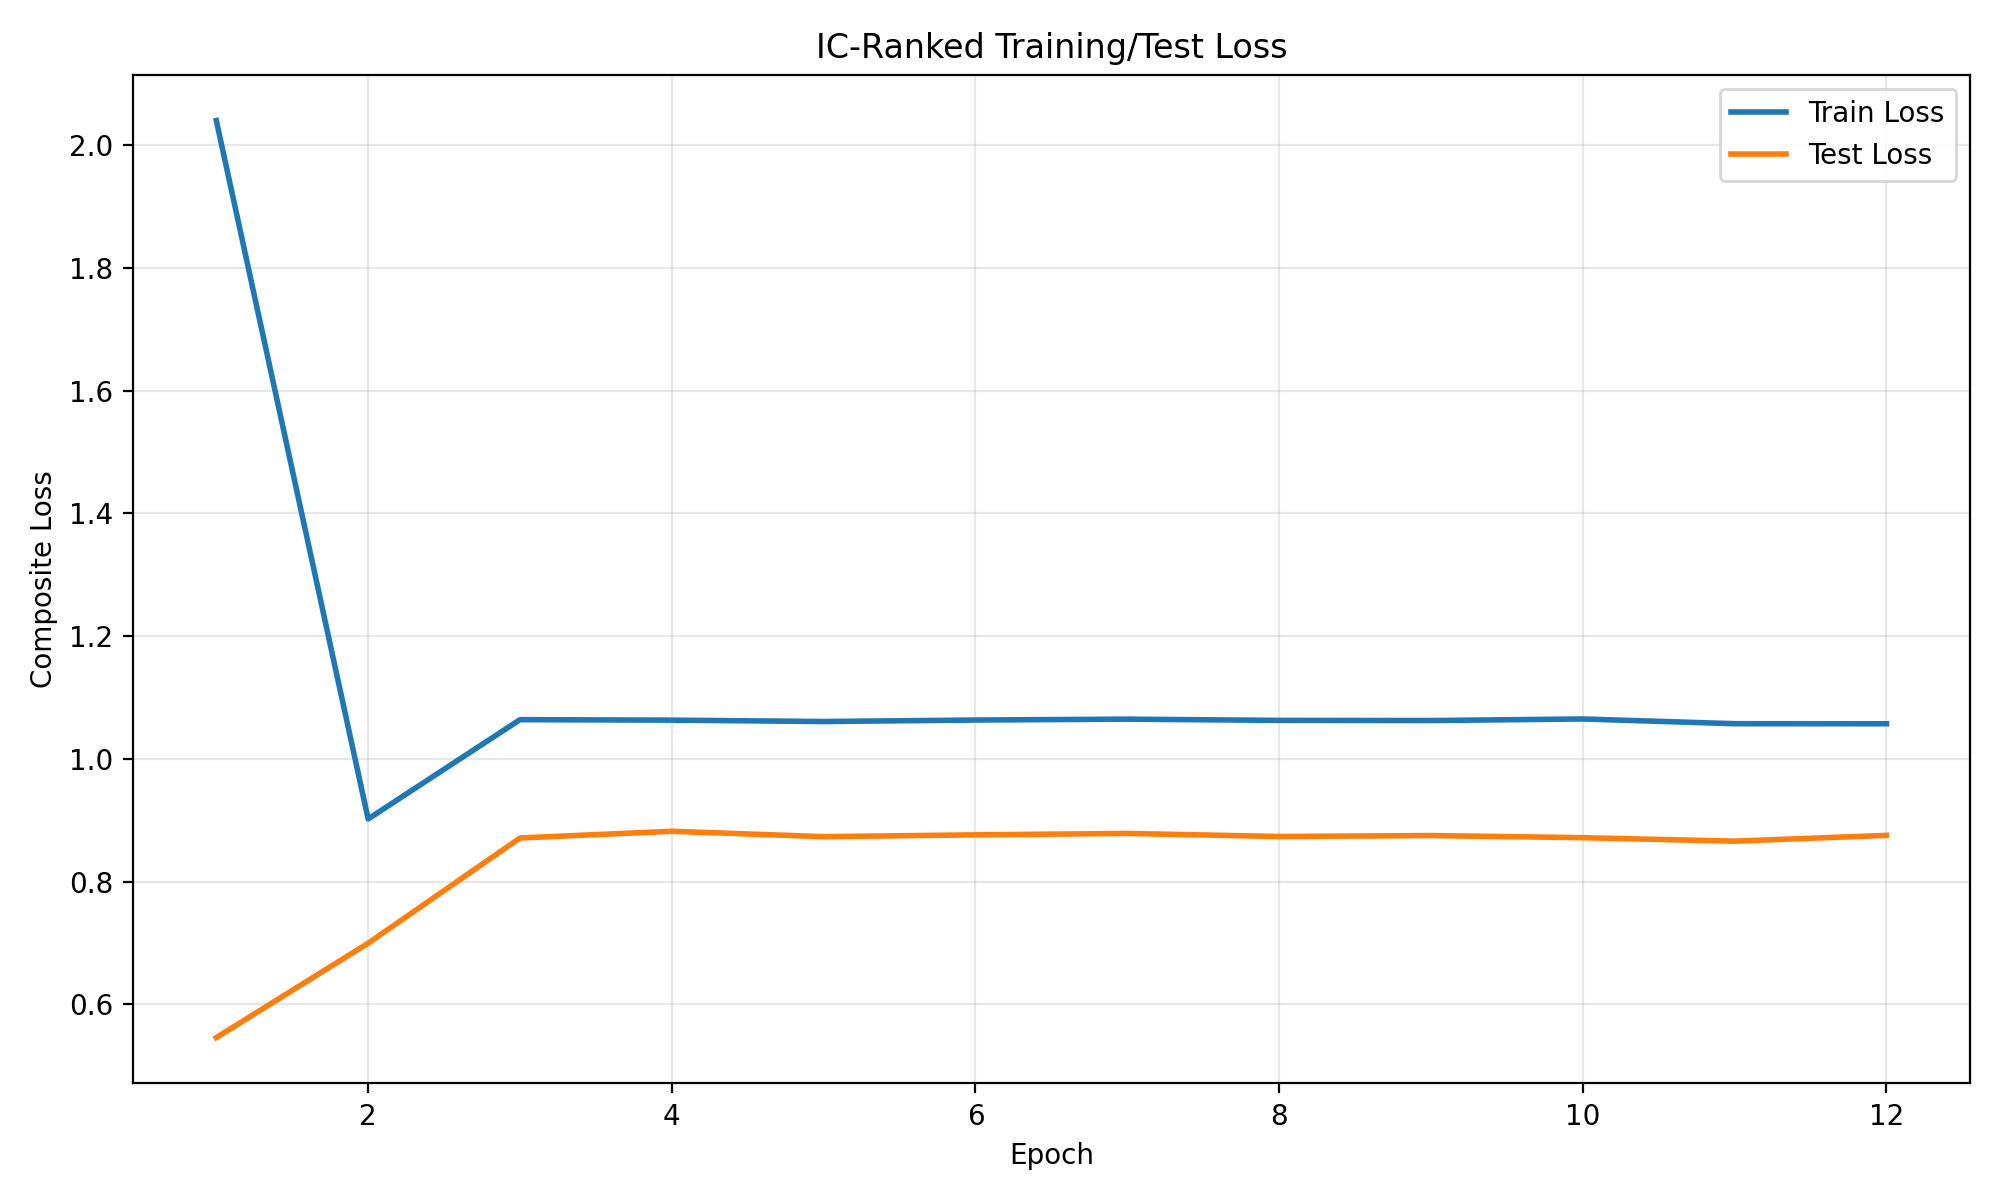
\includegraphics[width=\textwidth]{../data/plots/2024-12-31_icrank_loss_curve.png}

      \smallskip
      {\small Loss curves (MSE + IC + dispersion) for all three splits.
      IC warmup visible in the first 10 epochs.}
    \end{column}
  \end{columns}
\end{frame}

\begin{frame}{Live Predictions — March 2026}
  \begin{columns}[T]
    \begin{column}{0.48\textwidth}
      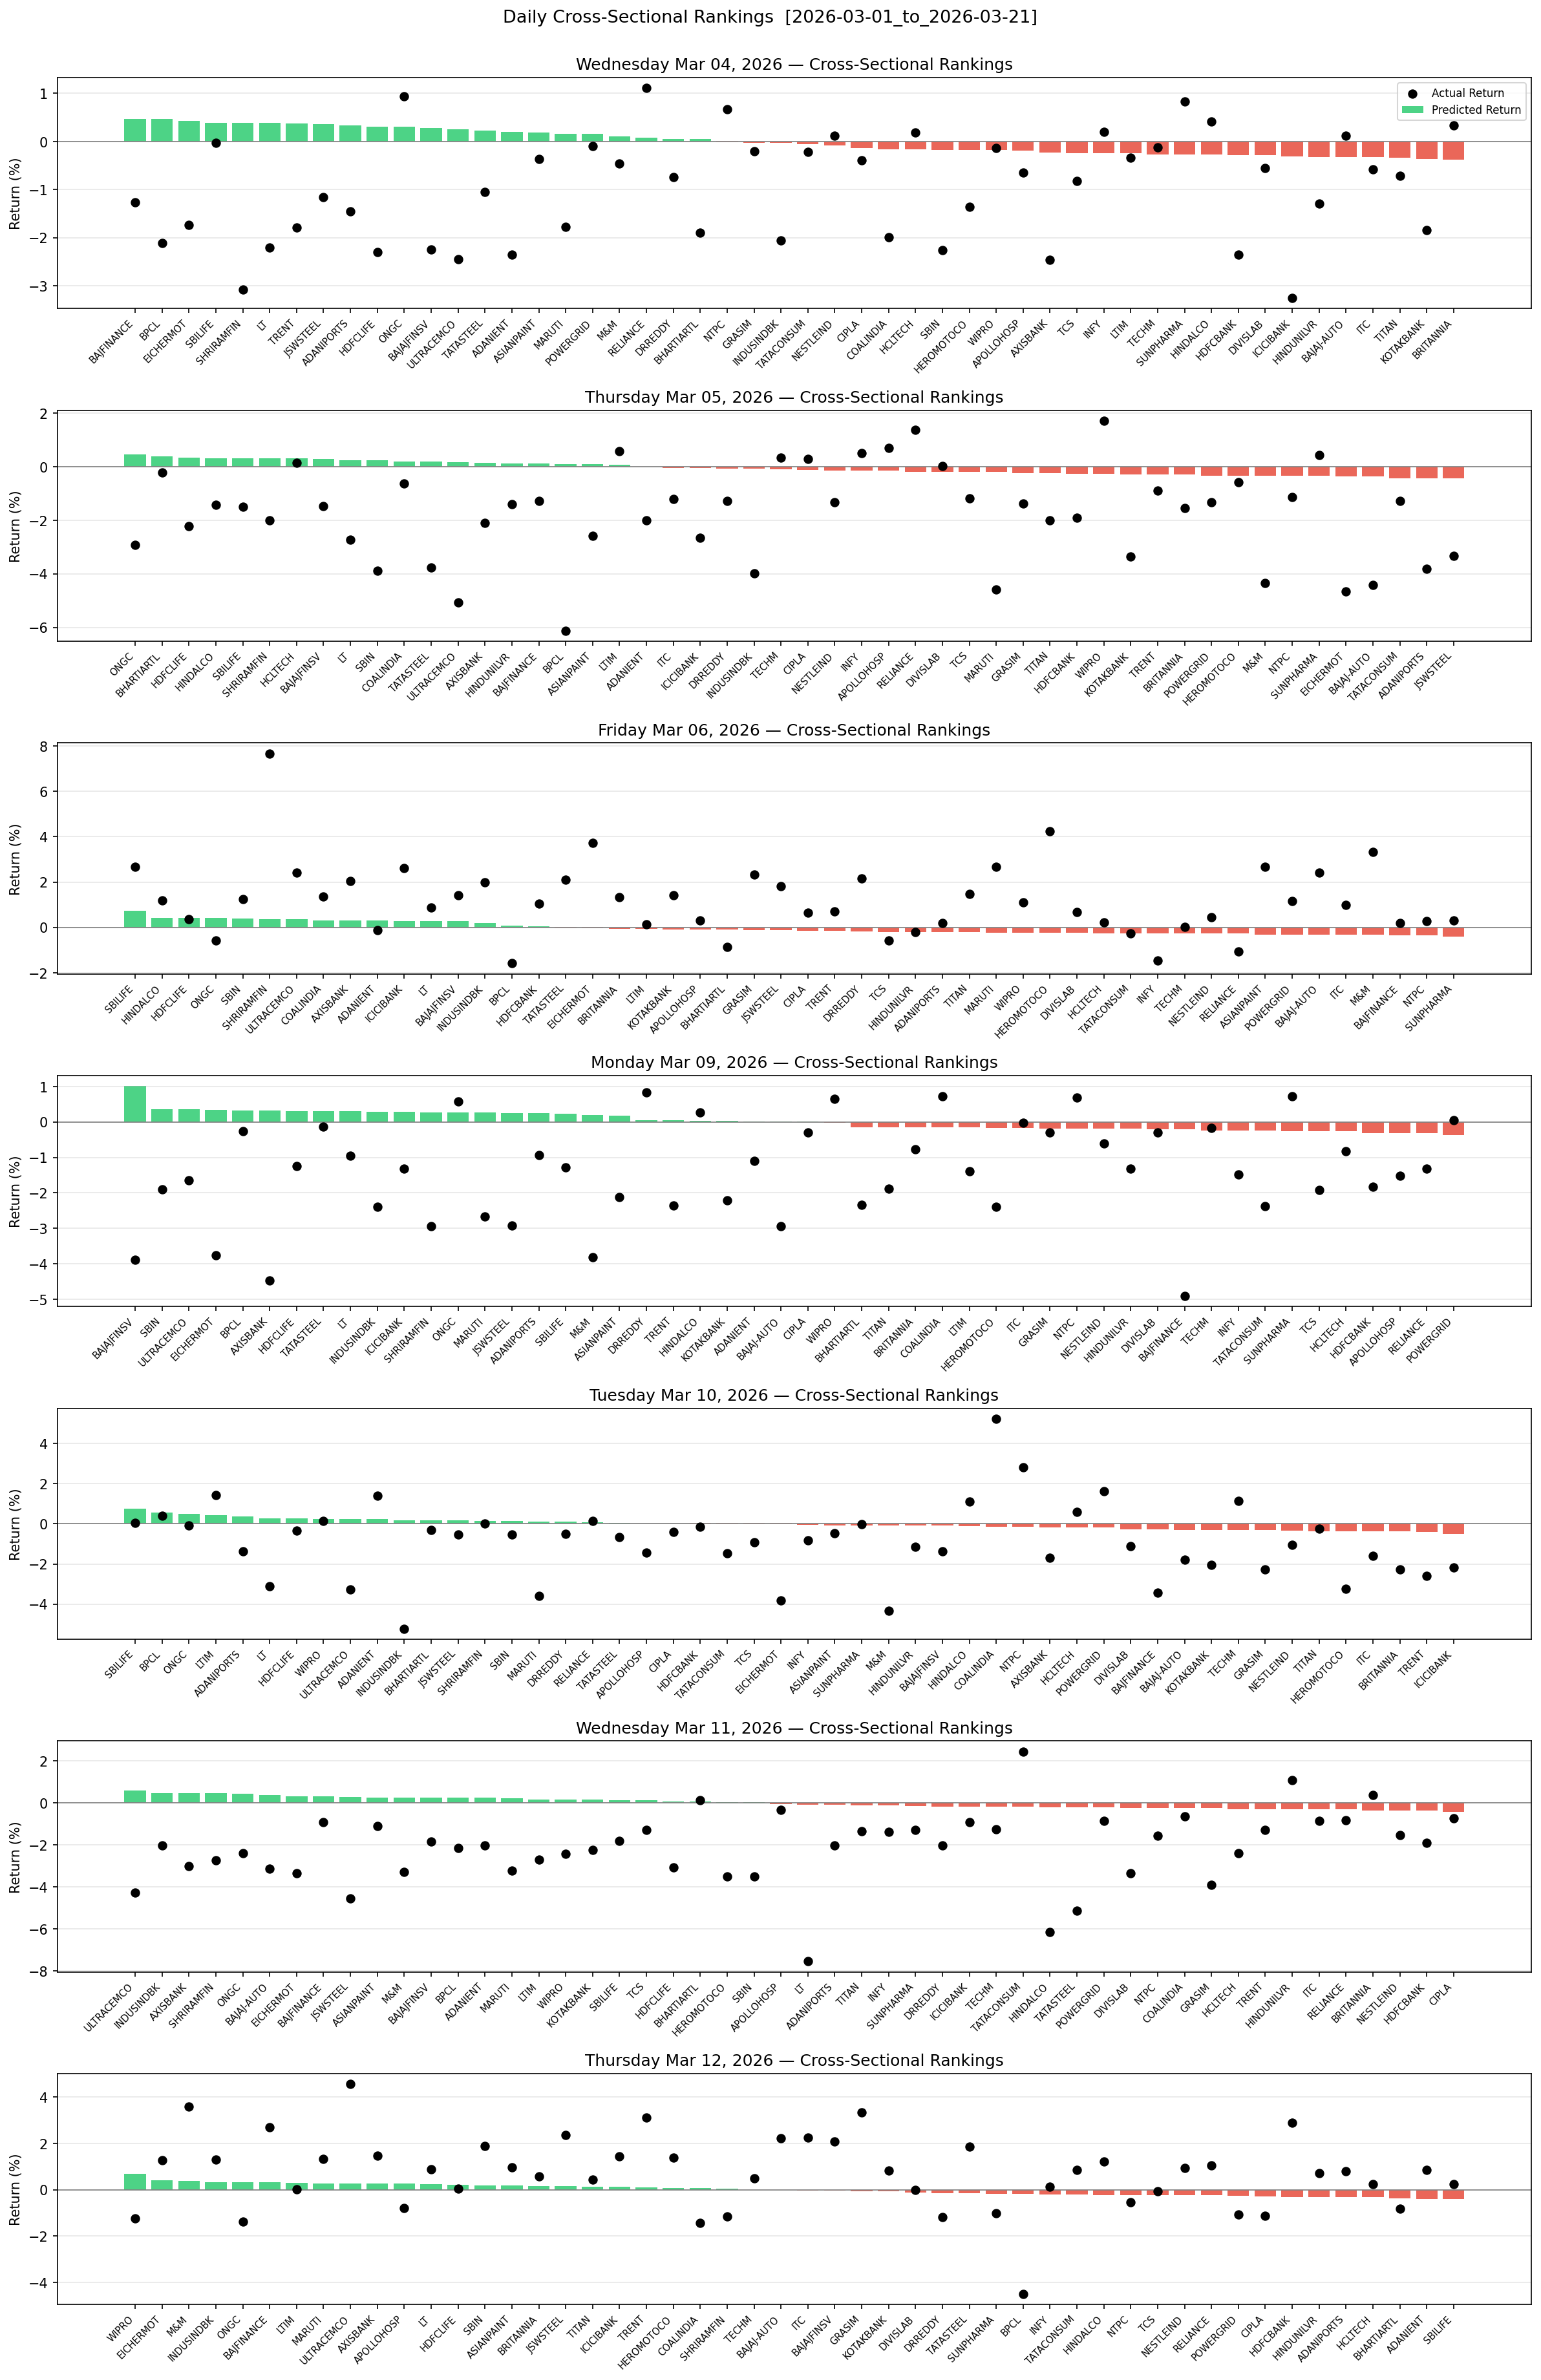
\includegraphics[width=\textwidth]{../data/plots/live_rankings_2026-03-01_to_2026-03-21.png}

      \smallskip
      {\small Predicted daily rankings across all 50 Nifty stocks.}
    \end{column}
    \begin{column}{0.48\textwidth}
      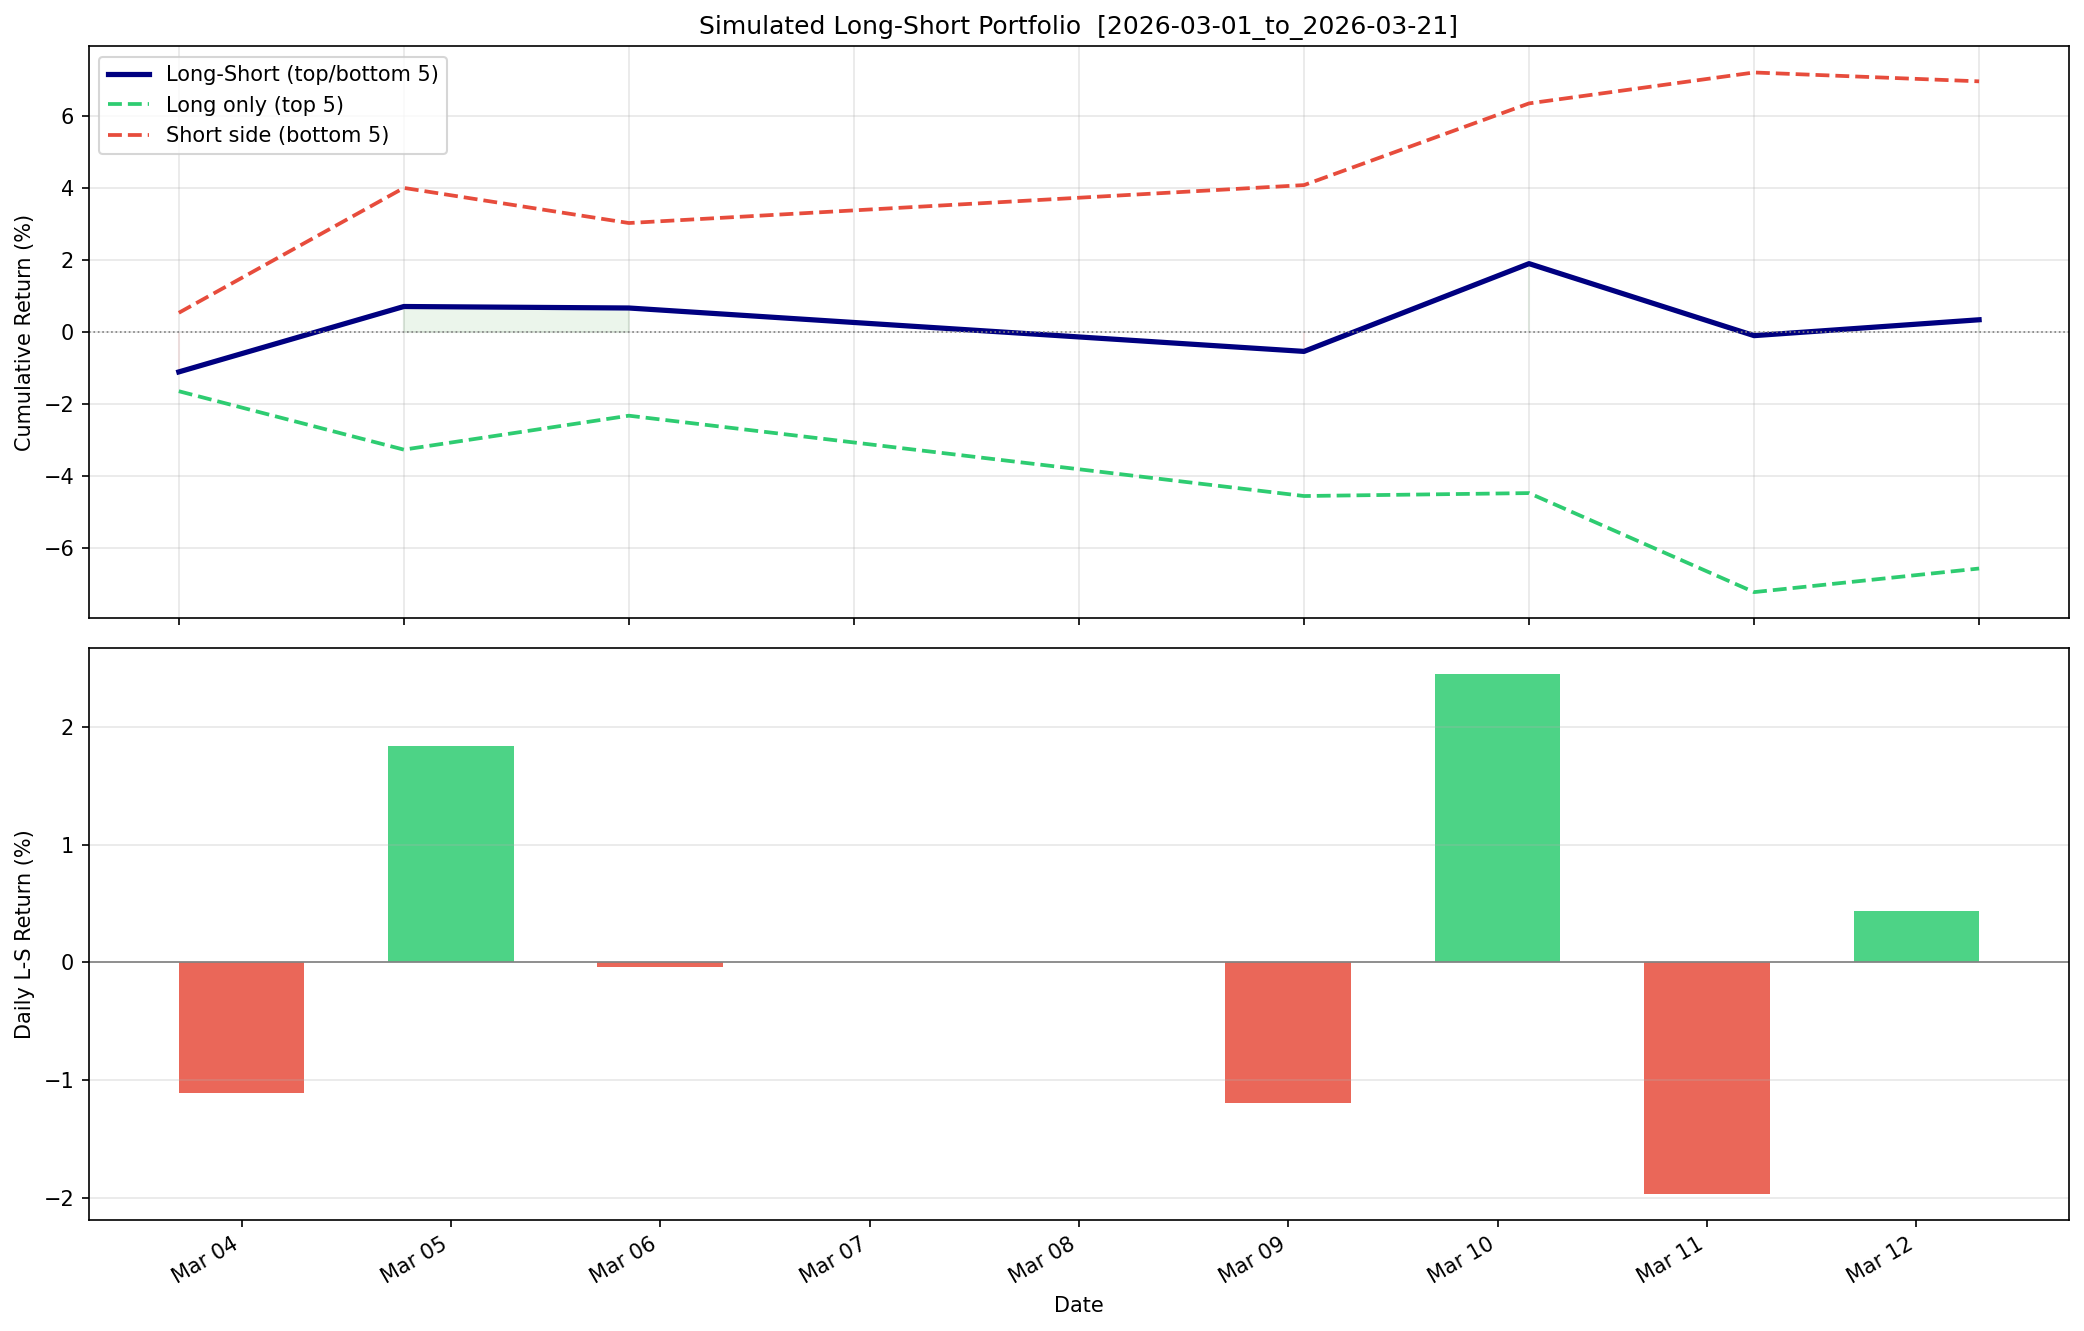
\includegraphics[width=\textwidth]{../data/plots/live_longshort_2026-03-01_to_2026-03-21.png}

      \smallskip
      {\small Long-short portfolio: top-5 minus bottom-5 cumulative return.}
    \end{column}
  \end{columns}
\end{frame}

\begin{frame}{Live Predictions — Individual Stocks}
  \begin{columns}[T]
    \begin{column}{0.48\textwidth}
      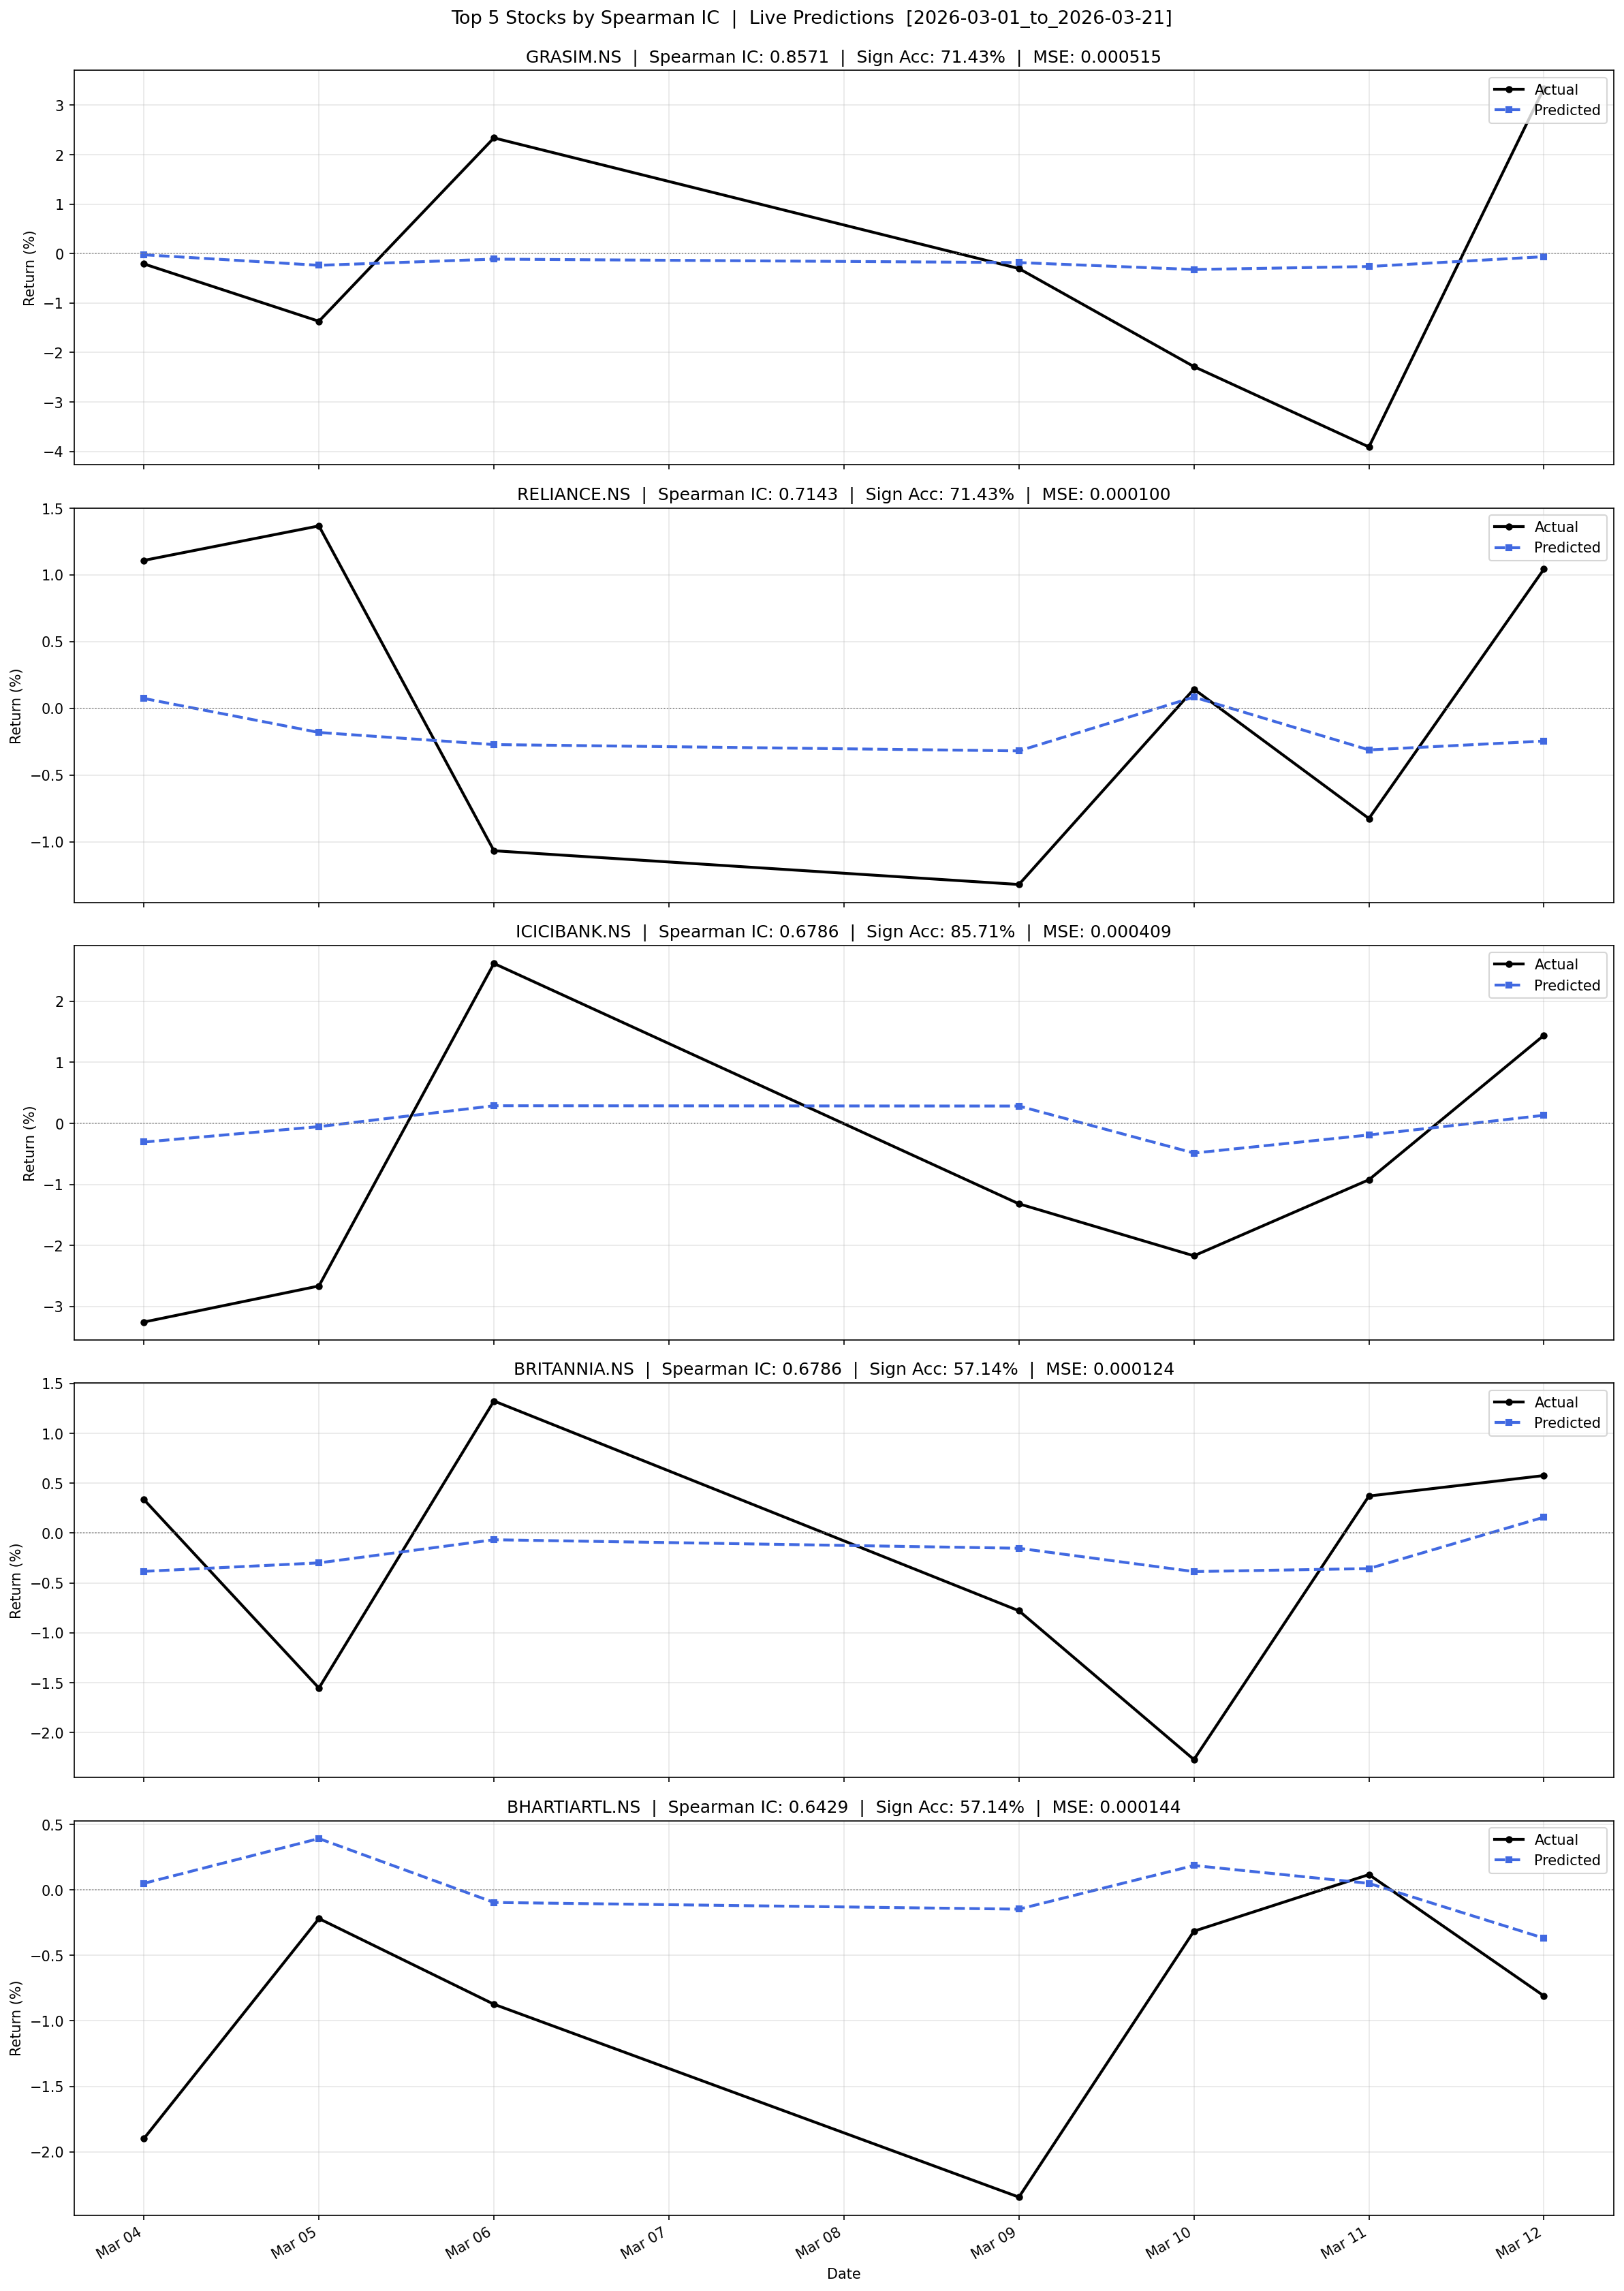
\includegraphics[width=\textwidth]{../data/plots/live_top5_2026-03-01_to_2026-03-21.png}

      \smallskip
      {\small Predicted vs.\ actual returns for top-5 ranked stocks.}
    \end{column}
    \begin{column}{0.48\textwidth}
      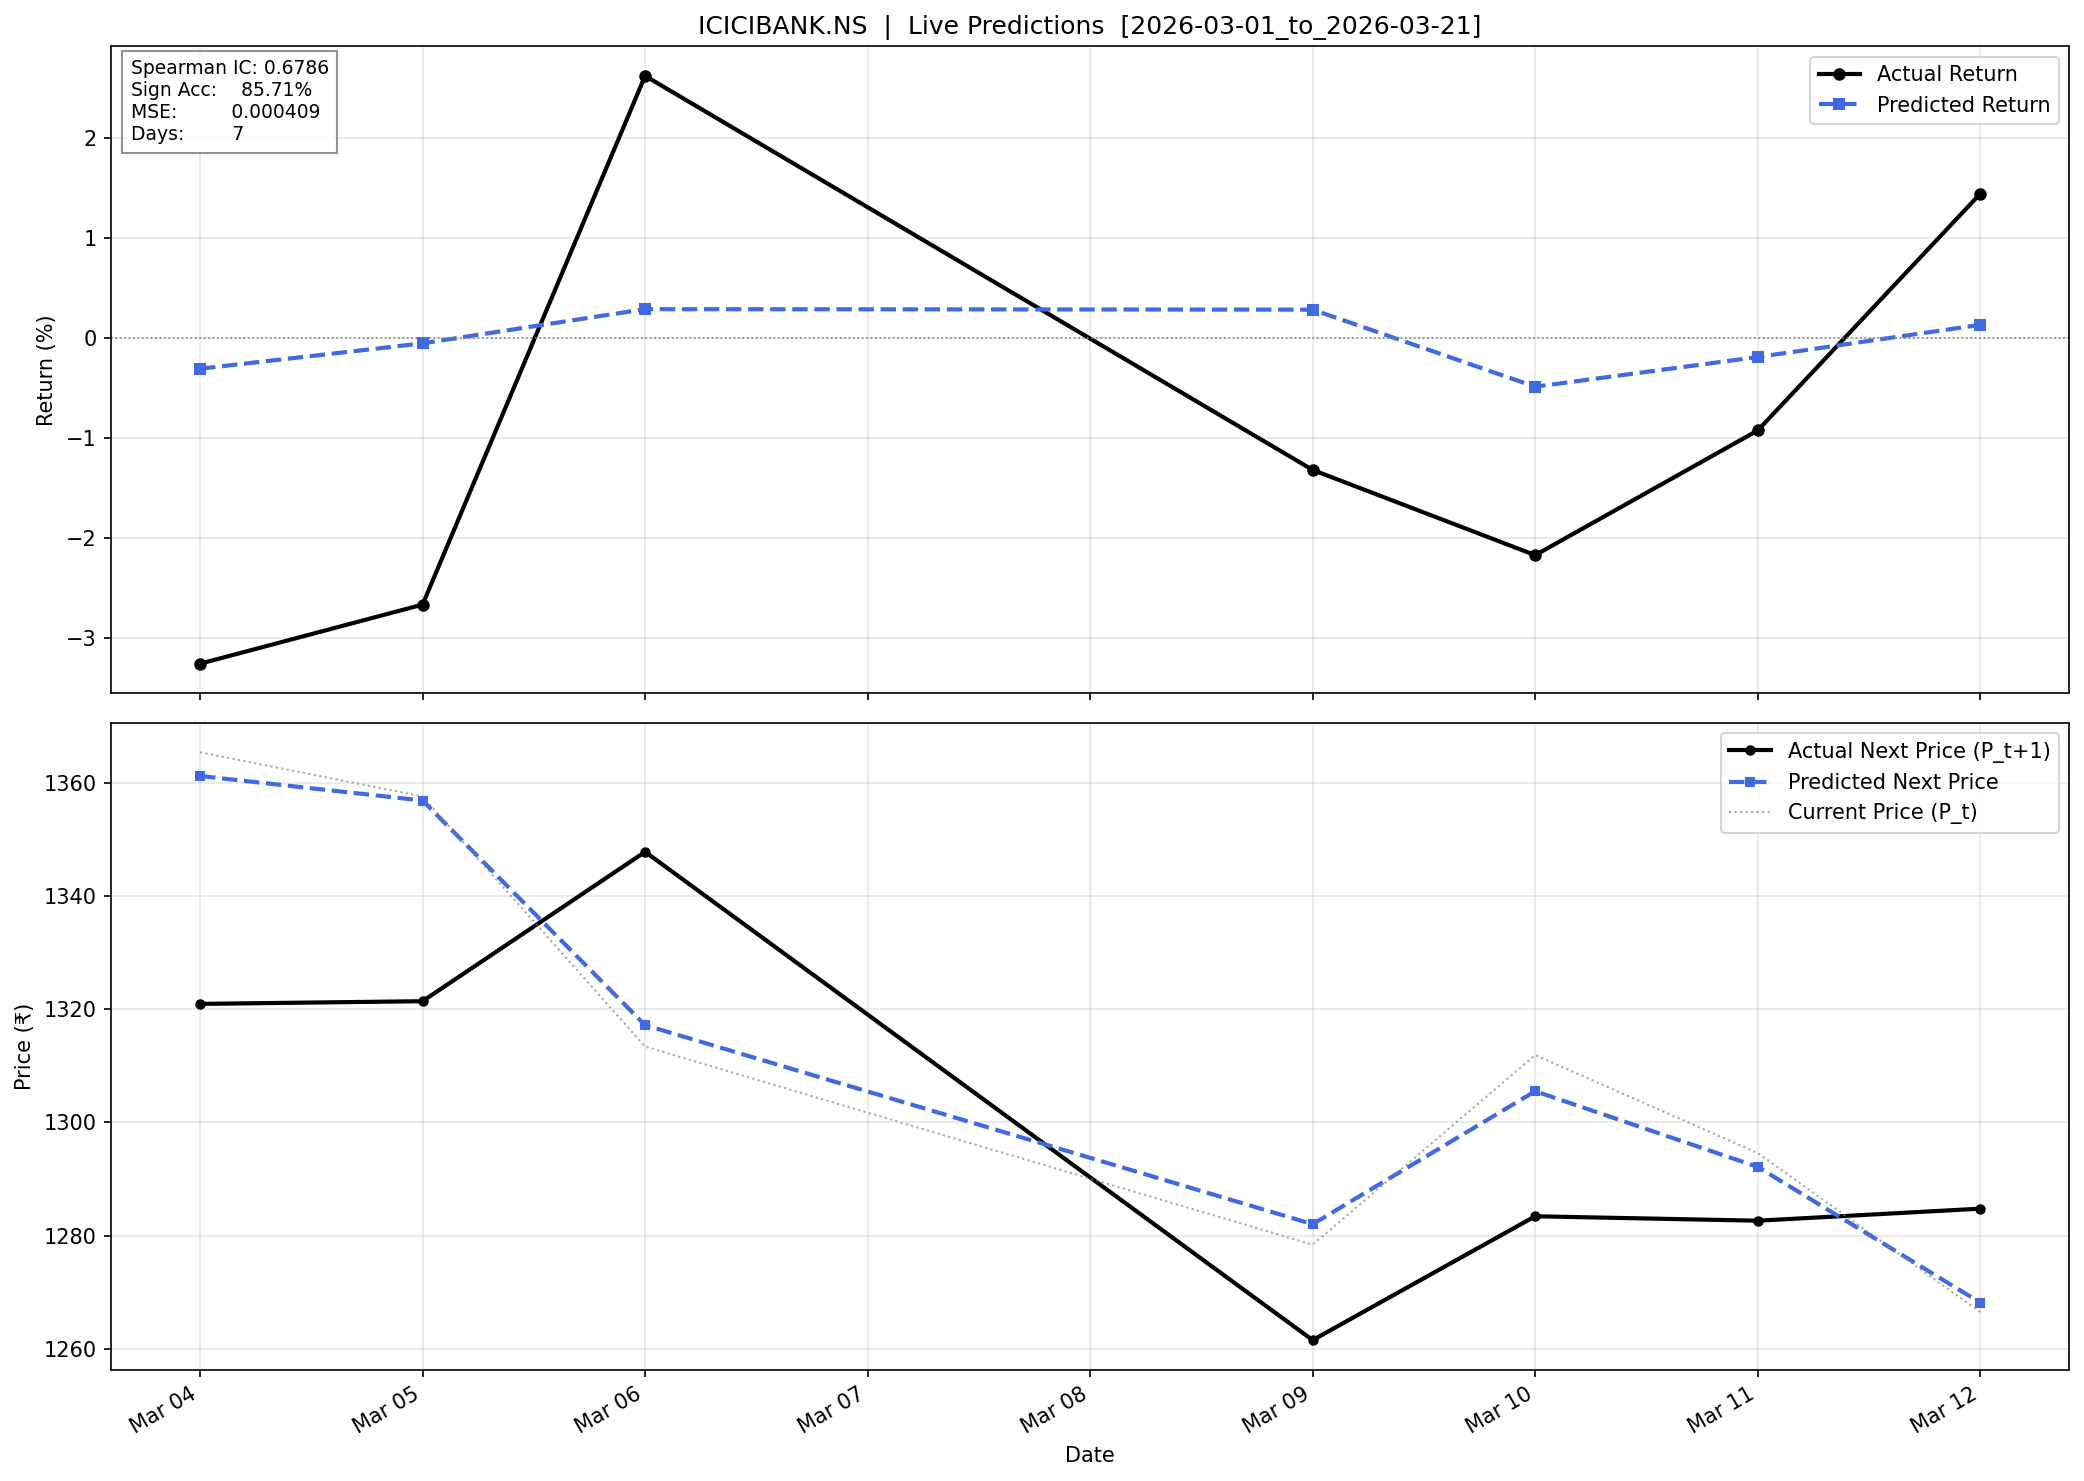
\includegraphics[width=\textwidth]{../data/plots/live_2026-03-01_to_2026-03-21_ICICIBANK.NS.png}

      \smallskip
      {\small ICICIBANK: predicted vs.\ actual next-day return.}
    \end{column}
  \end{columns}
\end{frame}

% ============================================================
\section{Limitations \& Future Work}
% ============================================================

\begin{frame}[shrink=12]{Current Limitations}
  \begin{columns}[T]
    \begin{column}{0.48\textwidth}
      \textbf{Architecture:}
      \begin{itemize}\setlength{\itemsep}{3pt}
        \item \textbf{Pairwise constraint}: can only model two-stock
              relationships; sector-wide shocks decomposed into pairwise
              edges lose higher-order signal
        \item \textbf{Static within a forward pass}: adjacency is
              recomputed daily but fixed during inference
        \item \textbf{GRU vs.\ Transformer}: GRU may under-capture
              long-range temporal dependencies compared to
              attention-based encoders
      \end{itemize}
    \end{column}
    \begin{column}{0.48\textwidth}
      \textbf{Training \& Data:}
      \begin{itemize}\setlength{\itemsep}{3pt}
        \item \textbf{Universe size}: 50 Nifty stocks only; does not
              generalise across index composition changes
        \item \textbf{Feature set}: 12 OHLCV + technical features; no
              macro, sentiment, or order-book features
        \item \textbf{Ranking objective}: MSE + soft-IC is not a pure
              profit-maximisation criterion (STHAN-SR addresses this)
        \item \textbf{Transaction costs}: live evaluation ignores
              slippage and market impact
      \end{itemize}
    \end{column}
  \end{columns}
\end{frame}

\begin{frame}[shrink=8]{Future Directions — Towards Hypergraph Architectures}
  \begin{columns}[T]
    \begin{column}{0.55\textwidth}
      \textbf{Short-term improvements to THGNN:}
      \begin{enumerate}\setlength{\itemsep}{3pt}
        \item Replace GRU with Transformer encoder (patch-based,
              like StockMixer)
        \item Add macro indicators as \emph{global} node features
        \item Walk-forward re-training with calendar rebalancing
      \end{enumerate}

      \medskip
      \textbf{Hypergraph extensions:}
      \begin{enumerate}\setlength{\itemsep}{3pt}
        \setcounter{enumi}{3}
        \item \textbf{STHAN-SR}: replace regression loss with
              learning-to-rank (ListNet / LambdaRank) for direct
              portfolio optimisation
        \item \textbf{MaGNet}: probabilistic hyperedges with soft
              stock membership across latent market themes
        \item Dynamic hyperedge discovery via spectral clustering on
              the time-varying correlation tensor
      \end{enumerate}
    \end{column}
    \begin{column}{0.42\textwidth}
      \begin{block}{Why Hypergraphs?}
        \begin{itemize}\setlength{\itemsep}{3pt}
          \item A single macro event (e.g.\ RBI rate change) affects an
                \emph{entire sector} simultaneously — this is a
                hyperedge, not pairwise edges
          \item Stocks belong to multiple \emph{overlapping} themes
                (e.g.\ HDFC is both banking and Nifty 50 constituent)
          \item Group-wise aggregation preserves higher-order market
                structure
        \end{itemize}
      \end{block}
    \end{column}
  \end{columns}
\end{frame}

% ============================================================
\section{Conclusion}
% ============================================================

\begin{frame}{Conclusion}
  \begin{columns}[T]
    \begin{column}{0.55\textwidth}
      \textbf{Contributions:}
      \begin{itemize}\setlength{\itemsep}{3pt}
        \item Full implementation of THGNN on Nifty 50 with dynamic,
              day-specific correlation graphs
        \item Composite IC-ranked loss (MSE + soft Spearman IC +
              dispersion) aligns training with portfolio ranking
        \item Heterogeneous pos/neg GAT distinguishes fundamentally
              different market relationship types
        \item Clean three-stage data pipeline reproducible from raw
              Yahoo Finance data
      \end{itemize}
    \end{column}
    \begin{column}{0.42\textwidth}
      \textbf{Key takeaways:}
      \begin{enumerate}\setlength{\itemsep}{3pt}
        \item Graph structure improves over independent-stock baselines
              by enabling information flow across correlated stocks
        \item Soft Spearman IC loss is more aligned with portfolio
              evaluation than pure MSE
        \item Pairwise GNNs remain limited — the next frontier is
              \textbf{hypergraph architectures} for group-wise dynamics
      \end{enumerate}

      \medskip
      \begin{block}{Best Val IC}
        \centering
        $\text{IC}_\text{val} = 0.029$\\
        {\small trained on 9 years of Nifty 50 data}
      \end{block}
    \end{column}
  \end{columns}
\end{frame}

% ---- Appendix -----------------------------------------------
\appendix

\begin{frame}{References}
  \begin{thebibliography}{9}
    \bibitem{thgnn2022}
      Xiang et al.\ (2022).
      \textit{Temporal and Heterogeneous Graph Neural Network for Financial
      Time Series Prediction.} CIKM 2022.
      \href{https://doi.org/10.1145/3511808.3557089}{doi:10.1145/3511808.3557089}

    \bibitem{master2023}
      Ma et al.\ (2023).
      \textit{MASTER: Market-Guided Stock Transformer for Stock Price
      Forecasting.} AAAI 2024.

    \bibitem{stockmixer2024}
      Zhang et al.\ (2024).
      \textit{StockMixer: A Simple Yet Strong MLP Mixer for Stock
      Price Forecasting.}

    \bibitem{sthan2021}
      Sawhney et al.\ (2021).
      \textit{Stock Selection via Spatiotemporal Hypergraph Attention
      Network: A Learning to Rank Approach.} AAAI 2021.

    \bibitem{magnet2022}
      \textit{MaGNet: Multi-scale Graph-Guided Attention Network for
      Stock Prediction.} 2022.

    \bibitem{pairnorm2020}
      Zhao et al.\ (2020).
      \textit{PairNorm: Tackling Oversmoothing in GNNs.} ICLR 2020.
  \end{thebibliography}
\end{frame}

\end{document}
